\documentclass[11pt,a4paper]{scrartcl}

\usepackage{gensymb}		% to display symbols like "º"
\usepackage{url}            % to display URLs
\usepackage{graphicx}       % include this line if your document contains figures
\usepackage{float}			% to place images in an arbitrary place
\usepackage{latexsym}     	% extra symbols including triangles
\usepackage{mathrsfs}      	% calygraphic letters, \mathscr
\usepackage{mathtools}
\usepackage{bm}              % bold greek letters
\usepackage{multicol}
\usepackage{subcaption}

\setkomafont{disposition}{\normalfont\bfseries}

\title{Path Planning and Robot Automatic Control and Navigatioon}
\subtitle{Robotics 2014/2015 \\ 2\textsuperscript{nd} Project}
\author{Duarte Paiva, Miguel Faria\\
		N\degree70751, N\degree73092\\
        duartemendespaiva@gmail.com, miguel.afonso.faria@gmail.com}
\date{June 5, 2015}

\def\SPSB#1#2{\rlap{\textsuperscript{#1}}\SB{#2}}
\def\SP#1{\textsuperscript{#1}}
\def\SB#1{\textsubscript{#1}}
\DeclarePairedDelimiter\abs{\lvert}{\rvert}
\DeclarePairedDelimiter\norm{\lVert}{\rVert}

\begin{document}
\maketitle
\newpage
\tableofcontents{}

\section{Introduction}

\subsection{Goals}
For this laboratory assignment, the goals were to:
\begin{itemize}
	\item plan a path from a point inside the laboratory and a point in the fifth floor and return to the laboratory;
    \item develop a program that guided a robot through the planned path, by using a control law, without the robot colliding with walls and obstacles that might exist in the path;
    \item in the developed program, integrate ways to deal with errors in odometry and sonar reads.
\end{itemize}

\subsection{Assumptions}
In this assignment, we assume that the obstacles along the path are static. In addition, we assume that the map used to plan the path is squared.

\subsection{Equipment}
For this assignment, we used MATLAB to generate the simulations and the program to control the robot. The robot used was a Pioneer P3-DX. %insert image here 

\section{Theoritical Fundaments}
The main principles behind this laboratory assignment were that to control a robot you need to create a model that can compensate local errors in the robot movement and eventually drive those errors to zero.\\
To do that, a control law must be created, which, based in the current data about the robot movement, decides the sequence of controls for the robot (linear velocity and angular velocity in this case) so it stays on course with minimal error.\\
Besides the control law, we also need to deal with errors in the sensors data that influence the results from the control law. To do that, it's important to understand how the robot moves and where we need to compensate sensors  errors, so the controls sent to the robot are the most correct.

\section{Referentials and Robot Model}
The robot referential is shown in figure \ref{fig:Robot_Referential}. According to that referential, if the robot is turning left its theta increments, and when turning right its theta decrements.
	\begin{figure}[H]
		\centerline{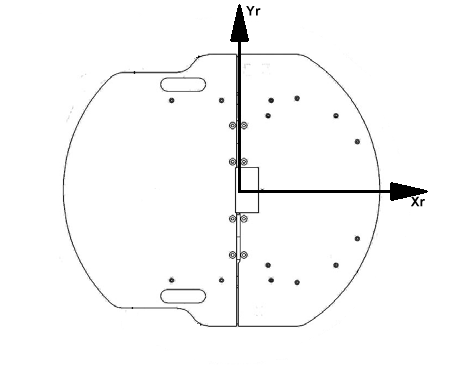
\includegraphics[width=0.5\textwidth]{pioneer_referential.png}}
    	\caption{Pioneer P3-DX referential.}
        \label{fig:Robot_Referential}
	\end{figure}

Besides taking into account the robot referential, we also had to set a referential for the map used in the simulations and used to control the physical robot movements. The map referential is shown in figure \ref{fig:Map_Referential}.

	\begin{figure}[H]
    	\centerline{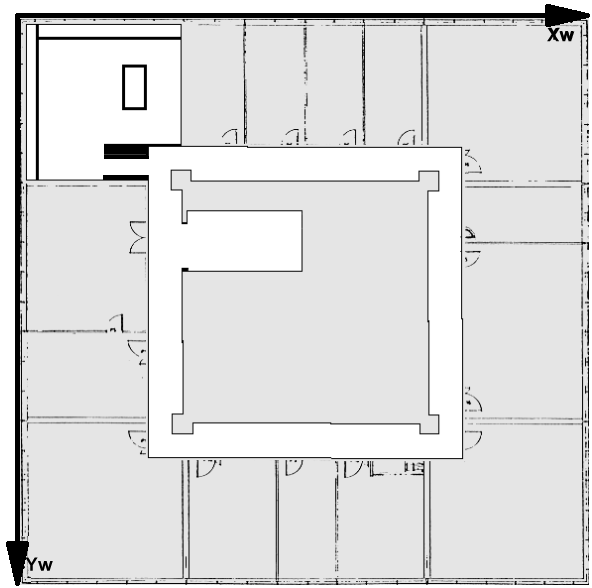
\includegraphics[width=0.5\textwidth]{map_referential.png}}
        \caption{Fifth floor map referential.}
		\label{fig:Map_Referential}
	\end{figure}

The robot initial position and orientation, in its own referential, is always (0,0,0\degree) and is always restarted when the robot is turned off and back on again. However the same isn't true regarding the physical environment referential (world referential). In this case, the robot initial position is given in reference to the world referential (0,0) point and the robot orientation in the world frame is given by the angle between the Xr and the Xw axes, being 0\degree  when both axes are aligned.

The Pionner P3-DX has a model that follows the unicycle robot model, so its movement can be described using the unicycle robot kinematic expressions:
	\[\begin{bmatrix}\dot{x}\\ \dot{y}\\ \dot{\theta} \end{bmatrix} = 
    	\begin{bmatrix} \cos(\theta) & 0\\ \sin(\theta) & 0\\ 0 & 1 \end{bmatrix} * 
        \begin{bmatrix} v \\ \omega \end{bmatrix}\]

Where \textit{v} stands for the linear velocity and $\omega$ for the angular velocity of the robot. With these expressions, it's possible to track the robot progression through the environment and see how far off trajectory the robot is and try to guide him back to the correct trajectory.\\
Those expressions also allow concluding that the robot used has some movement restraints: it's not possible for the robot to make a sideways movement, being necessary for it to rotate over its own axis and then move forward to perform an action similar to move to the side. This facts leads to extra considerations needing to be taken into account when designing a control program to make the robot follow a previously designed trajectory.

\section{Control Law}
The control law, as explained before, is a method through which the controls sent to the robot (in this case angular and linear velocities) are calculated in such a way that the error between the trajectory described by the robot and the reference trajectory goes to zero.

To solve the lab assignment we chose to implement a linear control law, since it was the one we concluded to have the best cost-benefit relation, since it was simple to implement and cost in work hours was less than with the other ones available. Following the material available in the class slides, we used the following expressions to compute the robot controls at each moment:
	\[u = \begin{bmatrix} -K\SB{1}e\SB{x} \\ -K\SB{2}sgn(v\SB{ref})e\SB{y} - K\SB{3}e\SB{$\theta$}\end{bmatrix}\]
    
Knowing that \textit{u} is the vector with the adjusts to the linear and angular reference velocities, and since we use constant linear velocity in the program to control the robot, the first line of \textit{u} can be ignored (it is applied to the linear velocity) and consequently K\SB{1} doesn't need to be determined.

However the same doesn't happen for K\SB{2} and K\SB{3}. Their value is calculated according to the following expressions:
	\[K\SB{2} = \frac{\omega\SPSB{2}{n} - \omega\SP{2}}{\abs{v\SB{ref}}} = b*\abs{v\SB{ref}}\]
    
    \[K\SB{3} = 2*\xi*\omega\SB{n} = 2*\xi*\sqrt{\omega\SPSB{2}{ref} + b*v\SPSB{2}{ref}}\]
    
The constants \textit{b} and \textit{$\xi$} were determined by experimentation, in both the simulation and field tests, trying to adjust them so the convergence on the reference trajectory was quick and smooth, driving the error to zero in a smooth way that would not originate other errors.

\section{Robot Control Program}
Our solution employs trajectory tracking to make the robot follow a trajectory specified by the user, so our program is composed by two distinct sections:
  \begin{enumerate}
      \item trajectory planning and generation;
      \item trajectory tracking using a linear control law.
  \end{enumerate}

\subsection{Trajectory Planning and Generation}
In the first part of the program the map of the environment is uploaded and the viable navigation points in the environment are calculated, generating a search tree with the possible navigable points. For that the map is subdivided into black areas (not navigable areas) and white areas (navigable areas). Whenever a division has mixed areas it is subdivided until it reaches a minimum dimension of 10x10 pixels. This was an arbitrary choice of minimum dimension and it was used to take in consideration a minimum area around the robot for its safe movement in the environment.

After this, the user gives a set of waypoints through which the robot must pass. Using the information from the previously computed tree and using a tree search algorithm called A*, the shortest path between each waypoint is determined, the determined points being the average points of each of the navigable areas.

After the major points in the trajectory are defined, we use pchip or spline (according to what the user chooses) to interpolate the path between each one of the trajectory points, creating the final trajectory that the robot must follow.

\subsection{Trajectory Tracking}
After the trajectory is computed, we start the trajectory tracking phase. This phase, basically, is a continuous loop that ends only when the robot achieves its objective or the user stops the program.

 Two main steps compose each iteration of the loop:
	\begin{itemize}
		\item robot localisation in the environment and error correction;
        \item obstacle avoidance and collision prevention;
	\end{itemize}

The basic scheme of each iteration is shown in figure \ref{fig:Tracking_Scheme}.

  \begin{figure}[H]
  	  \centerline{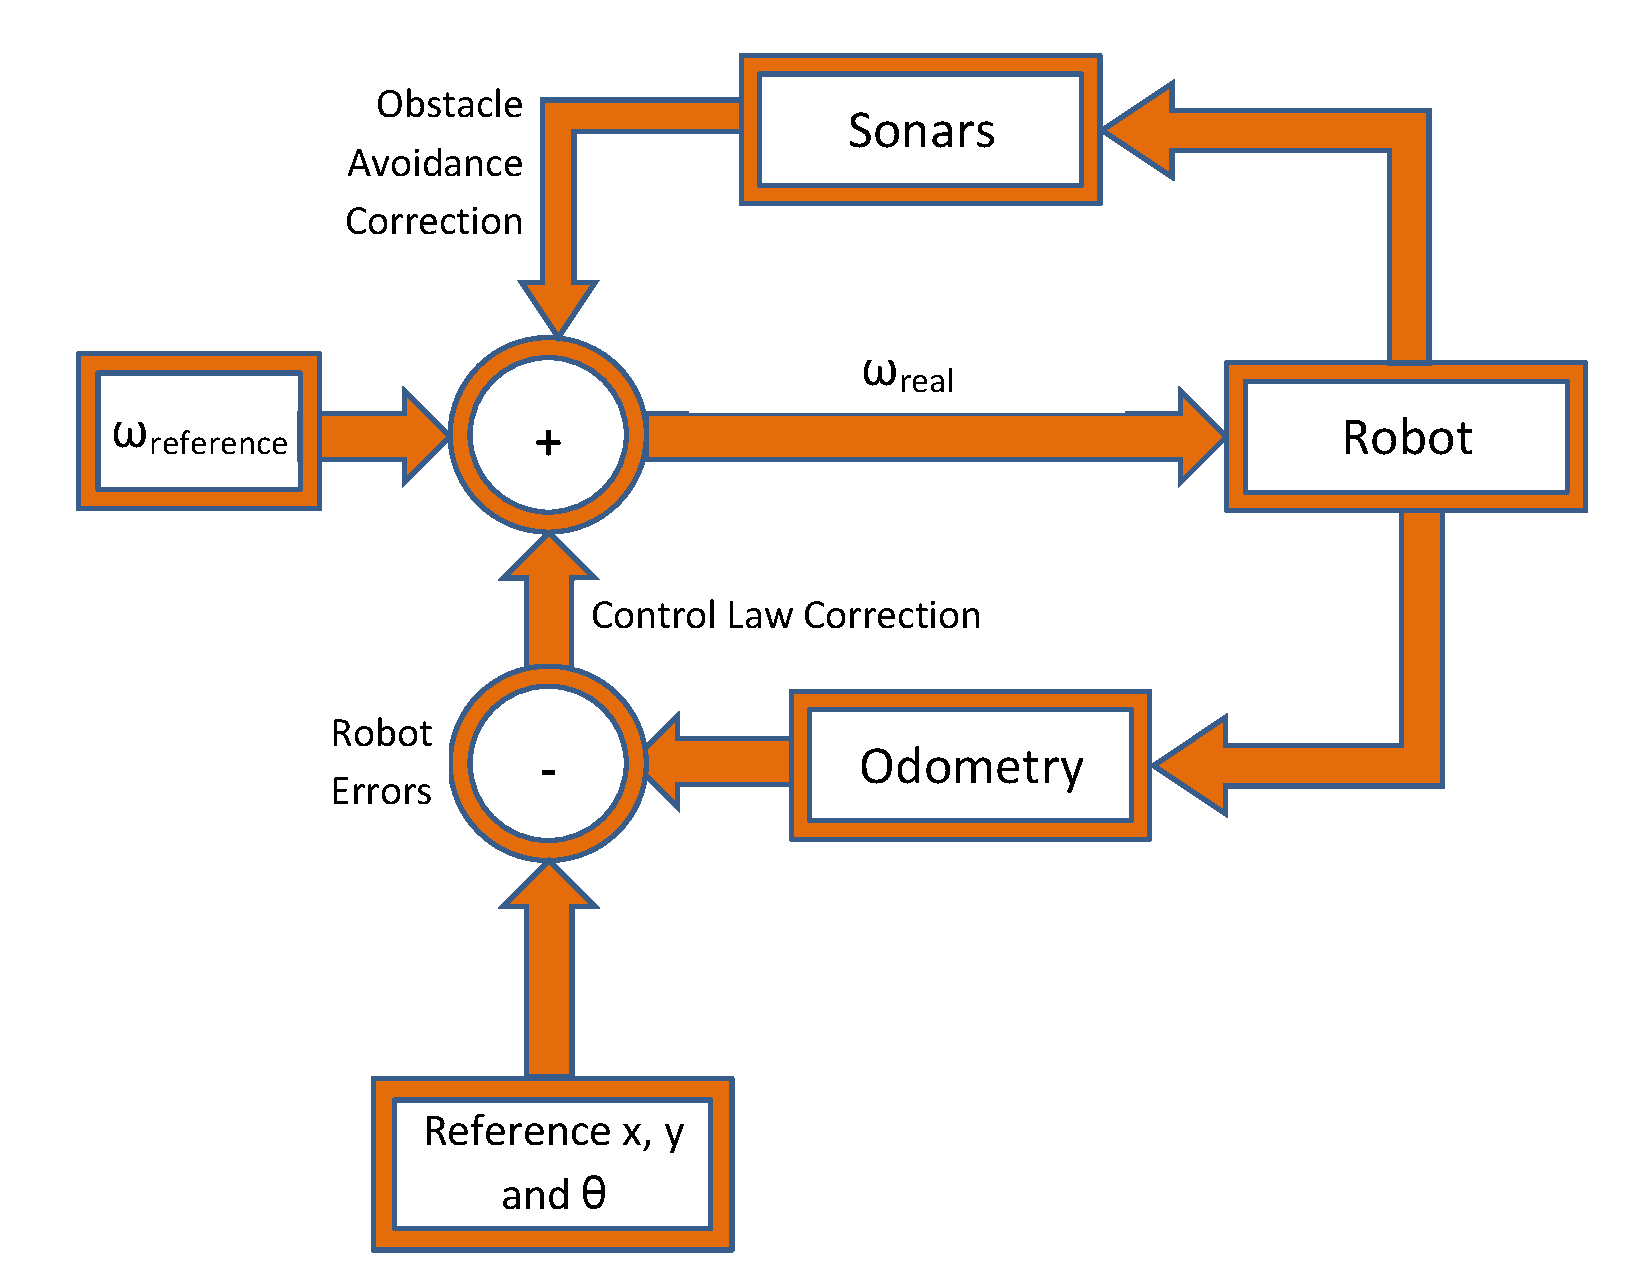
\includegraphics[width=0.5\textwidth]{Scheme.pdf}}
      \caption{Scheme of the trajectory tracking.}
      \label{fig:Tracking_Scheme}
  \end{figure}

\subsubsection{Robot Localisation and Error Correction}
In this step, we localise the robot by reading the odometry data in that moment and calculate where the robot is in relation to the starting point. Afterwards we run a basic search function on the reference trajectory to find the closest point of that trajectory to where the robot is localised.

With that information, we calculate the robot position error at that moment and, using the control law stated before, the adjustment to the angular velocity is calculated. 

One aspect that we had to take into consideration was that the odometry readings were subjected to errors originated by wheel slippage and inaccuracies in the odometry sensors. Thus, we had to compensate some errors in turns and define a maximum to the error to be taken into consideration when calculating the error correction.\\
As a result, whenever the robot described sharp turns we decelerated to reduce errors and compensated the angular velocity to prevent the robot from turning to much due to the slippage of the wheels. To compensate errors while moving in a straight line, we defined a maximum value for the robot errors and capped it when the errors were bigger than the limit, so the errors induced by the odometry wouldn't be of much significance.

Besides these errors, the wheels of the robot also weren't exactly equal and provoked slight deviations. These deviations were compensated using the sonars.

\subsubsection{Obstacle Avoidance and Collision Prevention}
In this step, we read the data from the sonars and check if the robot is close to any obstacle. For this, we created two danger levels and determined the danger distances, per sonar, to trigger the respective proximity alerts. The danger distances take in consideration each sonar location because the same distance represents different degrees of collision risk depending on the sonar location. The danger distances for each sonar are presented in table \ref{tab:sonar_distances}. 

	\begin{table}[H]
		\begin{center}
          \begin{tabular}{| c | c | c | c | c |}
              \hline Proximity Alert & 90\degree sonar & 50\degree sonar & 30\degree sonar & 10\degree sonar\\ \hline
              Level 1 & 450mm 		& 450mm 	& 450mm 	& 450mm \\ \hline
              Level 2 & 250mm 		& 350mm 	& 350mm 	& 350mm \\ \hline
          \end{tabular}
        \caption{Sonar Proximity Danger Distances}
        \label{tab:sonar_distances}
       	\end{center}
	\end{table}

With these danger levels we were able to create a hierarchy of reactions for the robot. When the robot recorded that one of the sonars entered a level one danger condition, the linear velocity of the robot would be reduced to half its initial velocity, so it would have time to correct its trajectory.

If the robot entered in a level two danger condition, then it would reduce the linear velocity to one quarter of its initial velocity and, also, would turn away from the obstacle according to the following expressions:
\[ sonar\_adjust = sonar\_adjust + (135 - abs(angle\_of\_sensor))*(level\_2\_distance - recorded\_distance)\]
\[ sonar\_adjust = sonar\_adjust - (135 - abs(angle\_of\_sensor))*(level\_2\_distance - recorded\_distance)\]

The first expression was used for the left side sonars and the second one for the right side sonars.

As it can be observed the \textit{sonar\_adjust} variable functions as an accumulator of the adjustment to the angular velocity due to the readings from the sonars. Because of that, we need to calculate the mean of the sum of the partial adjustments before using it to add to the adjustments to the angular velocity.

However, this method to prevent collisions can lead to multiple corrections in chain if the corrections done because of the sonars are too brusque. In this case, the robot may loose a little of its smooth movement.

\section{Experimental Results}
In this section we will present the results of our tests. First we will present the results of our tests for the simulation of the robot following the trajectory, and after we will show the main results for the tests done in the field, trying to complete a lap around the fifth floor of the North Tower of IST.

With the developed program, explained in the previous section, we wanted to fulfill the goals stated in the beginning of this report. With that in mind we now show the results of the tests conducted on our program, which will prove that the theoretical principles behind it are sound and that even though the full goal of this assignment was not met, the results achieved support the options we took and the viability of this program as a means to control the robot through a given reference trajectory.

\subsection{Simulation Results}
The simulation results show that the robot follows the reference trajectory very closely and recovers from errors quickly even after the sharpest turns. These results allow concluding that the program developed to control the robot, combined with the chosen control law, was an adequate choice and could provide the robot a correct sequence of commands so that the robot follows the trajectory with minimal error.

As evidence of these conclusions we present figures \ref{fig:Simulation_Map} and \ref{fig:Simulation_Map_Fixed} (showing in blue the reference trajectory and in red the robot trajectory), where it is possible to observe the stated conclusions. In figure \ref{fig:Simulation_Map} we can see how the simulation behaves with point interpolation using pchip. This is an interesting test because it allowed us seeing how the program behaves when the trajectories aren't built with equally spaced points and so the results give a better feel of how the program will work in the field.

	\begin{figure}[H]
      \centering
      \begin{subfigure}{.5\textwidth}
          \centering
          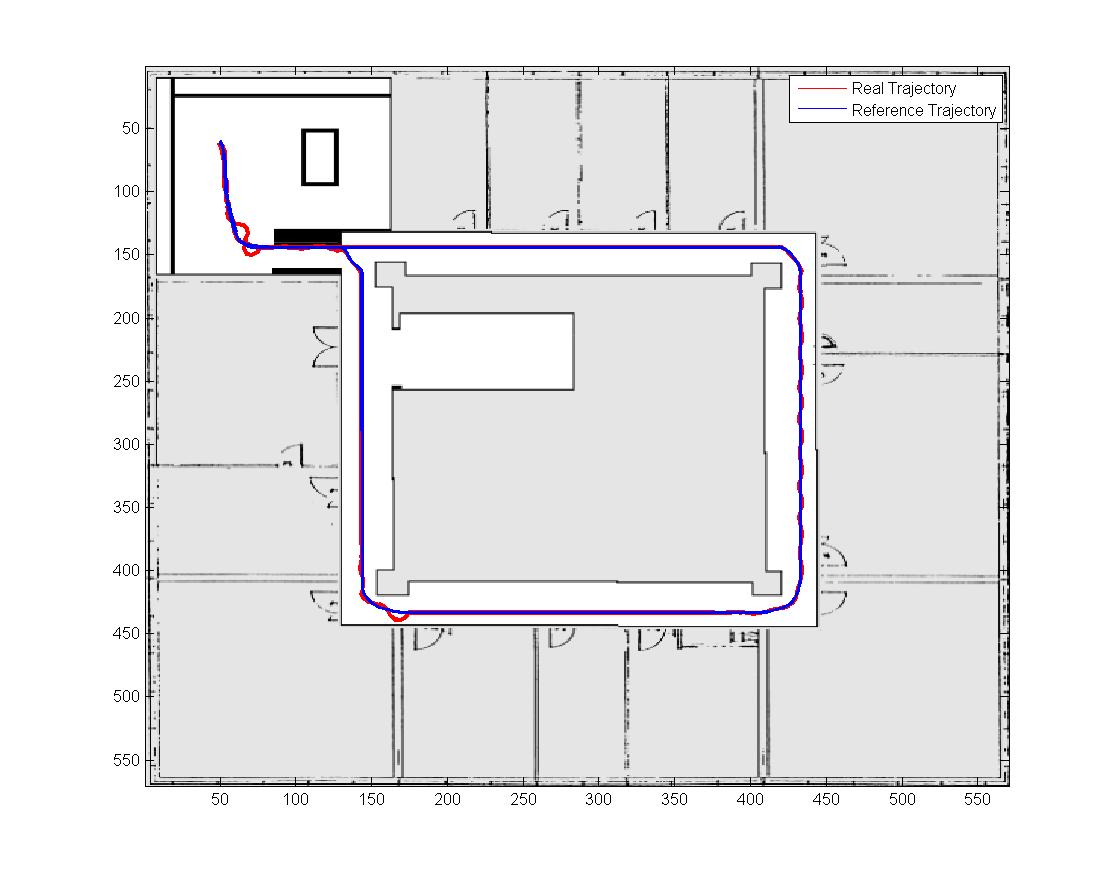
\includegraphics[width=0.7\linewidth]{simulation_map.jpg}
          \caption{Simulation Results for a trajectory given by the user with point interpolation.}
          \label{fig:Simulation_Map}
      \end{subfigure}%
      \begin{subfigure}{.5\textwidth}
          \centering
          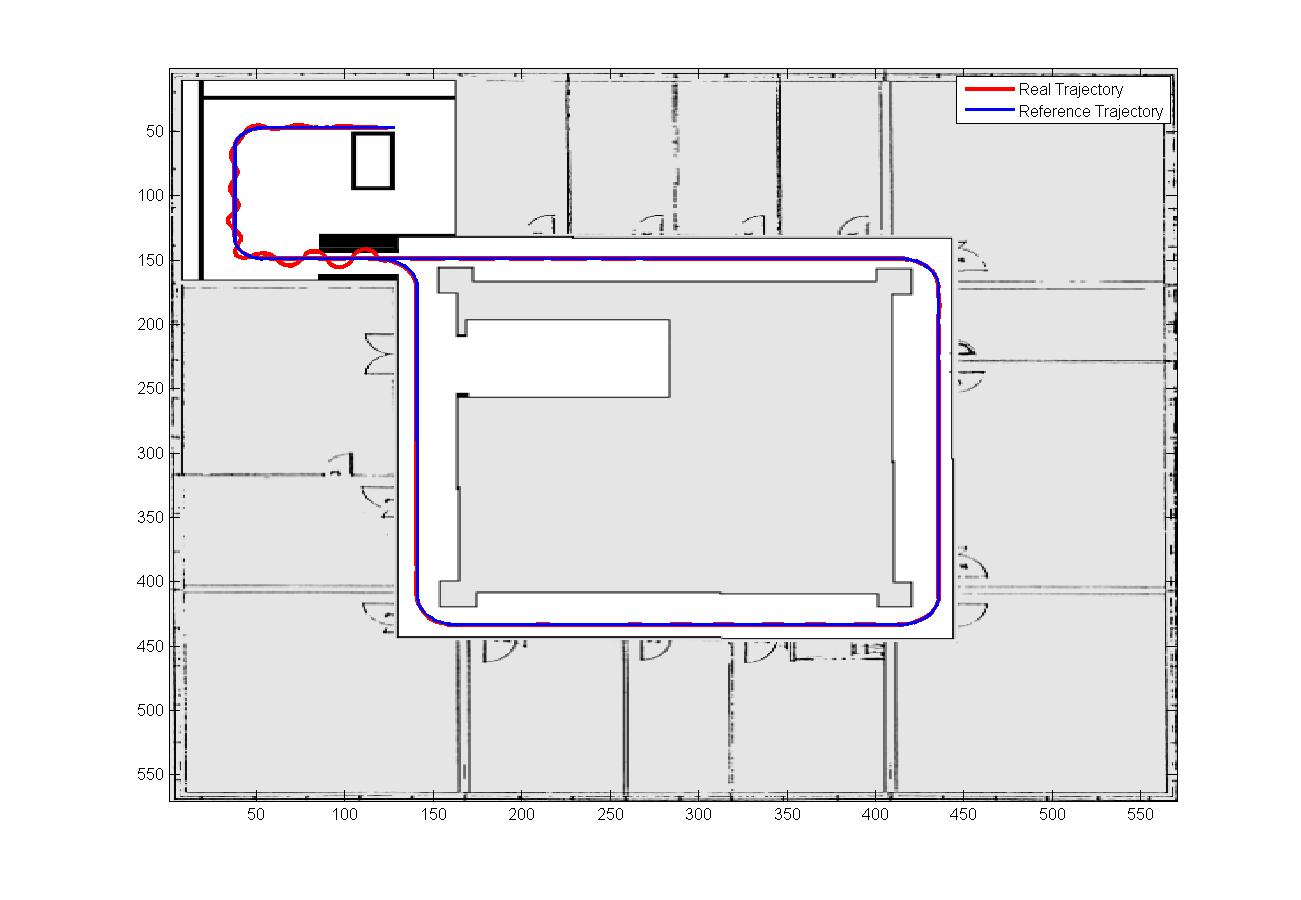
\includegraphics[width=0.7\linewidth]{simulation_map_fixed.jpg}
          \caption{Simulation Results for a trajectory built using exact measures and with no point interpolation.}
          \label{fig:Simulation_Map_Fixed}
      \end{subfigure}
	\end{figure}

In figure \ref{fig:Simulation_Map_Fixed} we see the results for a simulation with a well behaved trajectory, where the points are all equally spaced and the turns are very neat and perfect, a characteristic that doesn't occur with point interpolation. This kind of test served as the baseline when we applied major changes to our program.

Together with minimal error between the robot actual trajectory and the reference trajectory, it's also important to have a smooth convergence of the angular velocity to the reference angular velocity and that their difference is also small. Otherwise the robot would execute the trajectory correctly but with a small zig-zag which, besides not giving a natural feel to the movement, also would create a greater wear down of the robot's mechanical components.

On figures \ref{fig:simulation_velocities} and \ref{fig:simulation_velocities_fixed} we show the comparison between the reference angular velocity and the robot angular velocity (reference velocity in blue and robot velocity in red) for the same two tests shown before.

	\begin{figure}[H]
      \centering
      \begin{subfigure}{.5\textwidth}
          \centering
          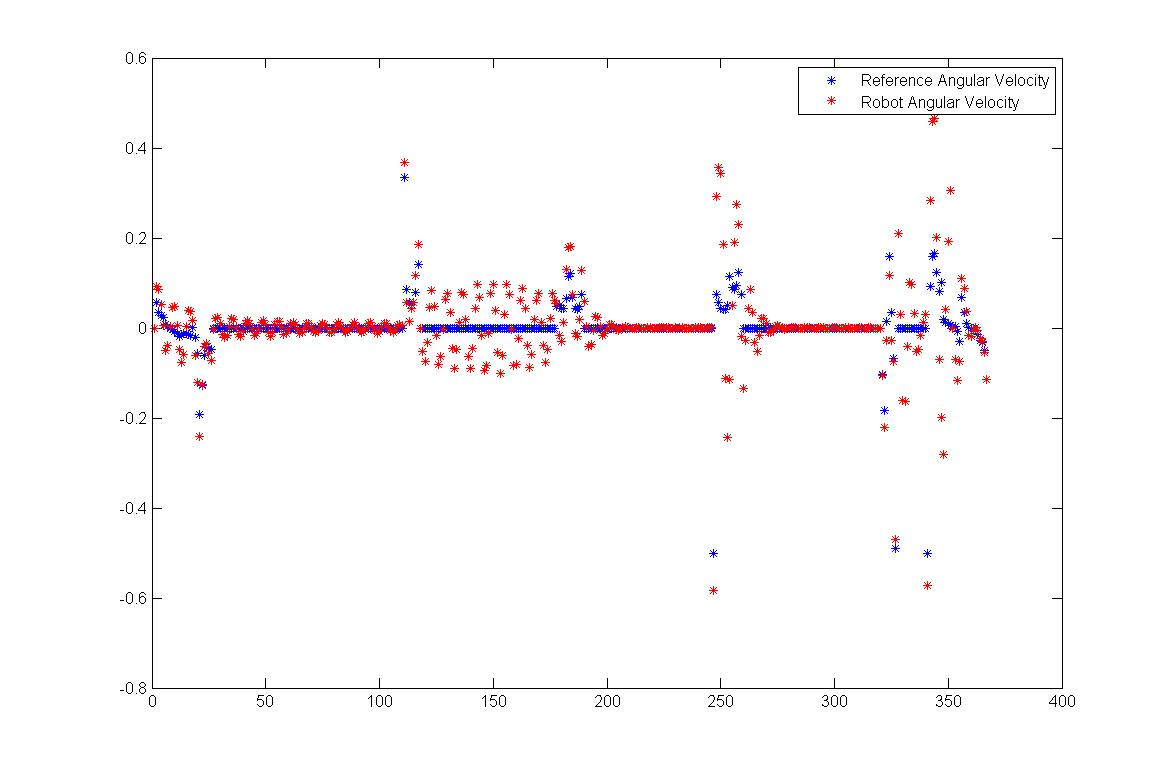
\includegraphics[width=0.7\linewidth]{simulation_velocities.jpg}
          \caption{Angular Velocities comparison for the test with point interpolation.}
          \label{fig:simulation_velocities}
      \end{subfigure}%
      \begin{subfigure}{.5\textwidth}
          \centering
          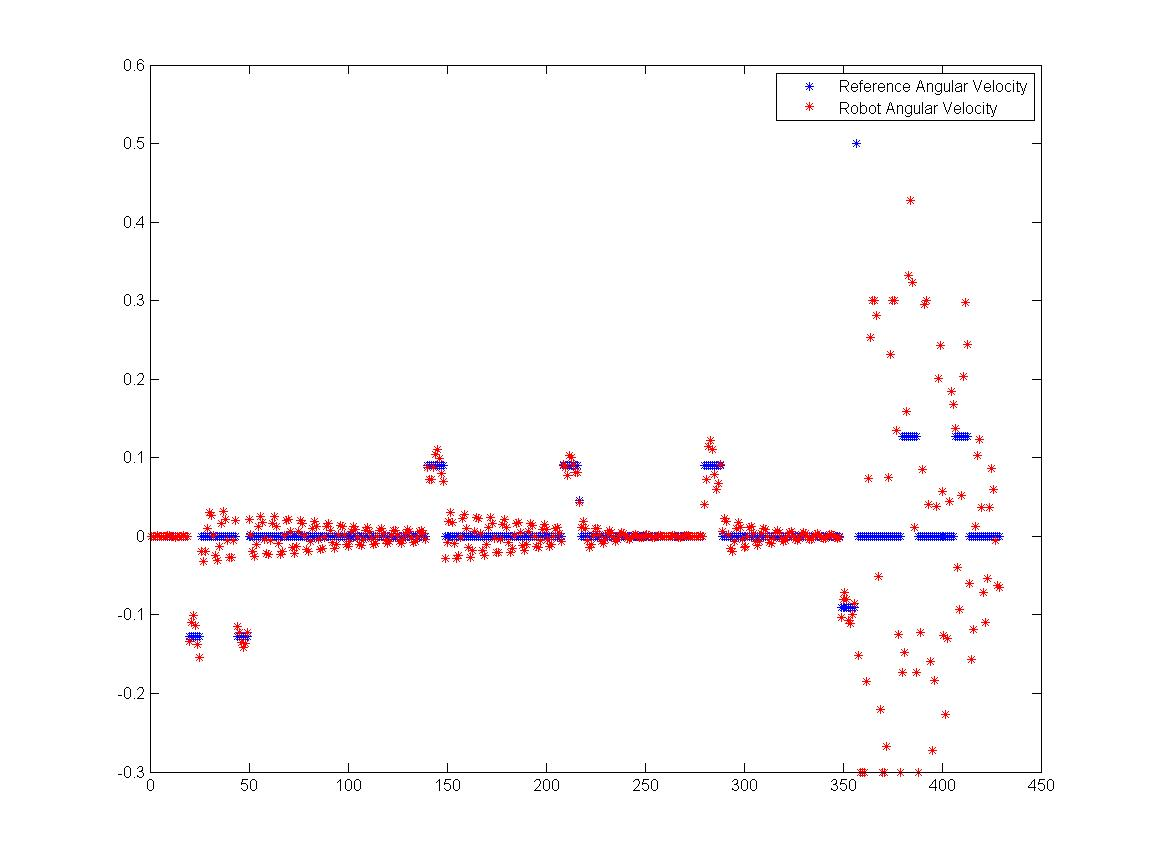
\includegraphics[width=0.7\linewidth]{simulation_velocities_fixed.jpg}
          \caption{Angular Velocities comparison for the test without point interpolation.}
          \label{fig:simulation_velocities_fixed}
      \end{subfigure}
	\end{figure}

As we can conclude from the previous figures, the robot angular velocity converges smoothly and quickly to the reference angular velocity and, when the robot starts to turn, the error increases but then it rapidly returns to match the reference values.

After analysing these results, we can conclude that the simulation shows a good performance of the developed control program with smooth and fast convergence to the reference trajectory and with small deviations from the trajectory once they converge. In addition, the robot angular velocity has a similar behaviour which is one of the aspects we aim for so that the robot can have a natural feel while moving, and also reduce wear of its mechanisms.

With these results we can prove that the theoretical bases of our program are solid and that the program is a good viable option to be implemented to control a robot of this kind, because the goals stated previously were achieved.

\subsection{Field Test Results}
The field test results weren't as good as the simulation results. Contrary to the results of the simulations, in the field tests the robot had many difficulties returning to the lab and never got back to the starting point.

Most of the times the robot reached the forth corridor and, although sometimes the robot would deviate from the trajectory so much it would go against a wall, it was able to reach the door of the laboratory. However, when it entered the last corridor, it was 2 m ahead of the point defined in the reference trajectory; so, the robot wasn't able to enter the laboratory.

In figure \ref{fig:field_test_result} we show the path executed by the robot, in one of the tests in which it reached the laboratory, when it was following the trajectory showed in figure \ref{fig:field_test_reference_trajectory}. 

	\begin{figure}[H]
      \centering
      \begin{subfigure}{.5\textwidth}
          \centering
          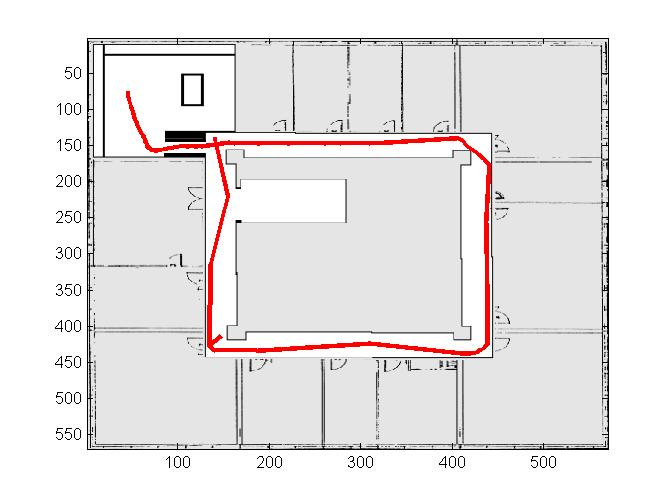
\includegraphics[width=0.7\linewidth]{field_test_robot_trajectory.jpg}
          \caption{Robot real trajectory during one of the tests it reached the door.}
          \label{fig:field_test_result}
      \end{subfigure}%
      \begin{subfigure}{.5\textwidth}
          \centering
          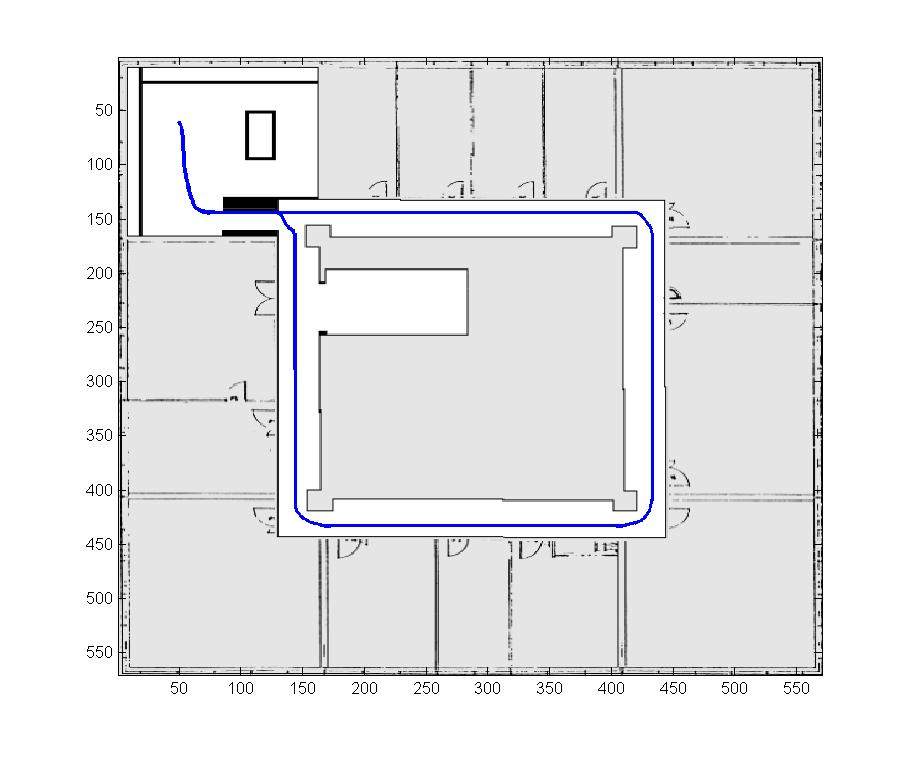
\includegraphics[width=0.7\linewidth]{field_test_reference_trajectory.jpg}
          \caption{Reference trajectory used to test the robot control program.}
          \label{fig:field_test_reference_trajectory}
      \end{subfigure}
	\end{figure}

	\begin{figure}[H]
        \centering
        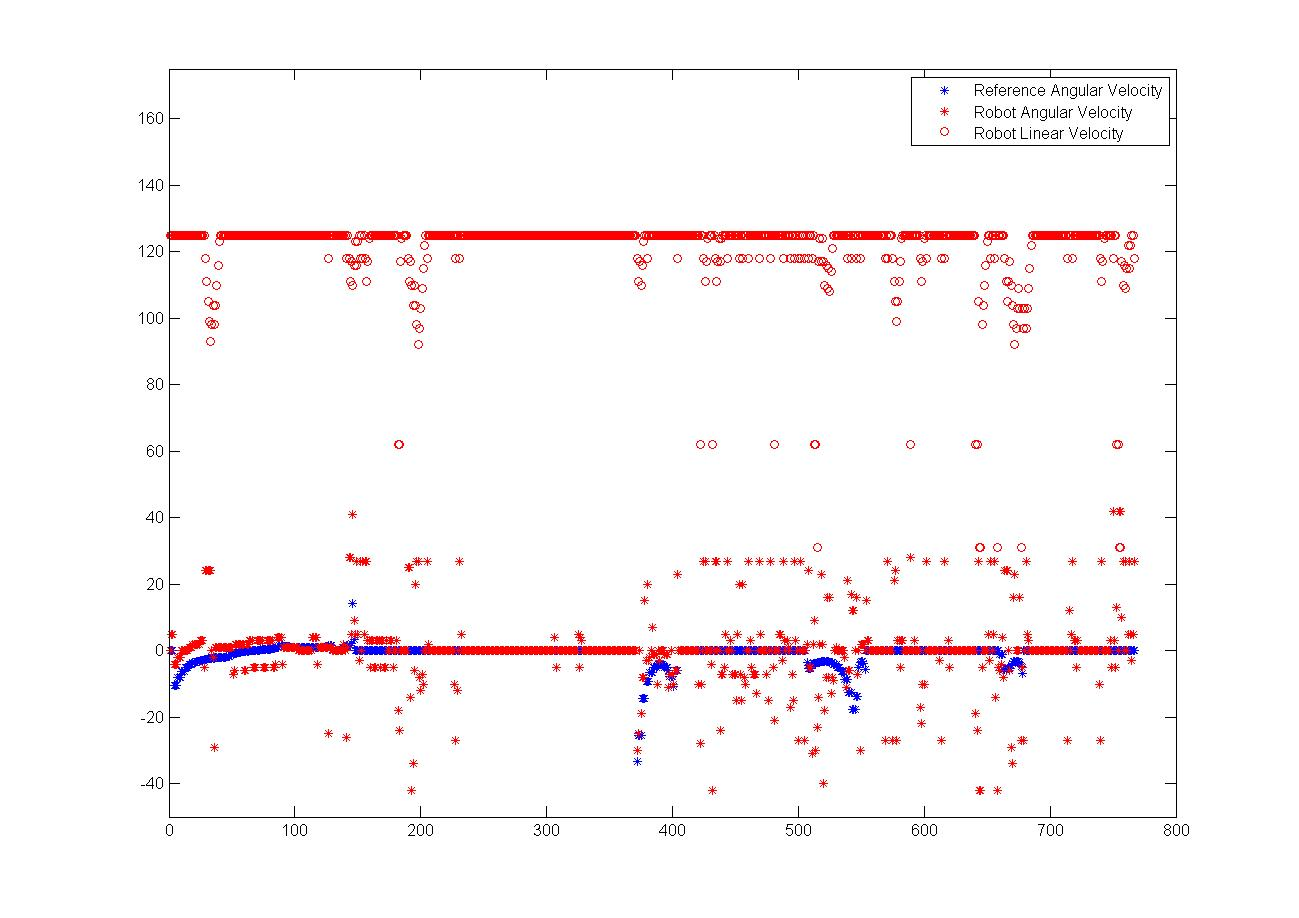
\includegraphics[width=0.7\linewidth]{field_test_velocities.jpg}
        \caption{Recorded Robot Angular and Linear Velocities during the test.}
        \label{fig:field_test_velocities}
    \end{figure}

In figure \ref{fig:field_test_velocities} we can see the velocities sent to the robot and how the robot decelerates when it has to make a sharp turn, accelerating again until top speed when it finishes the turn.

As we can see from the previous figures, the robot reached the laboratory door, but it entered few times. In fact our best results were that the robot would enter but would hit some closet or wall when it entered. In the test showed here the robot never hit any wall, but we stopped it when the robot started to move in circles instead of advancing.

These results were due to the fact that the robot was around 2 m ahead of the point it was using as reference (so it continued to move forward) and to that the laboratory entrance has some corners that reflect the sonars (the robot is always receiving signals that it is close to some obstacle, so it goes on turning trying to avoid hitting it).

One other aspect can be concluded from these results: if we compare the robot real trajectory against the reference, we see that sometimes the robot deviates from the reference even when it has already converged. This is due to the existence of obstacles in the environment around the robot that weren't considered when planning the trajectory and so the robot has to make some corrections to avoid colliding with them. These corrections are brusquer when the sonar data only recognizes the obstacle too late, thus the robot has to make sharper turns to prevent colliding. This delay in the detection occurs because of two main reasons:
\begin{itemize}
	\item the obstacles, when hit by a sonar signal, tend to reflect it in several directions and sometimes the reflected wave doesn't go directly to the sonar that emitted it, causing that the sonar receives an erroneous response that leads it to answer incorrectly;
    \item there is a time gap between the sonars emitting a signal and getting a response so, when they get it, the robot is close to the obstacle and has to turn more to prevent colliding.
\end{itemize}

In figure \ref{fig:sonar_map} we can see how the angular velocity of the robot changes with the data that the robot receives from the sonars.
\begin{figure}[H]
	\centering
	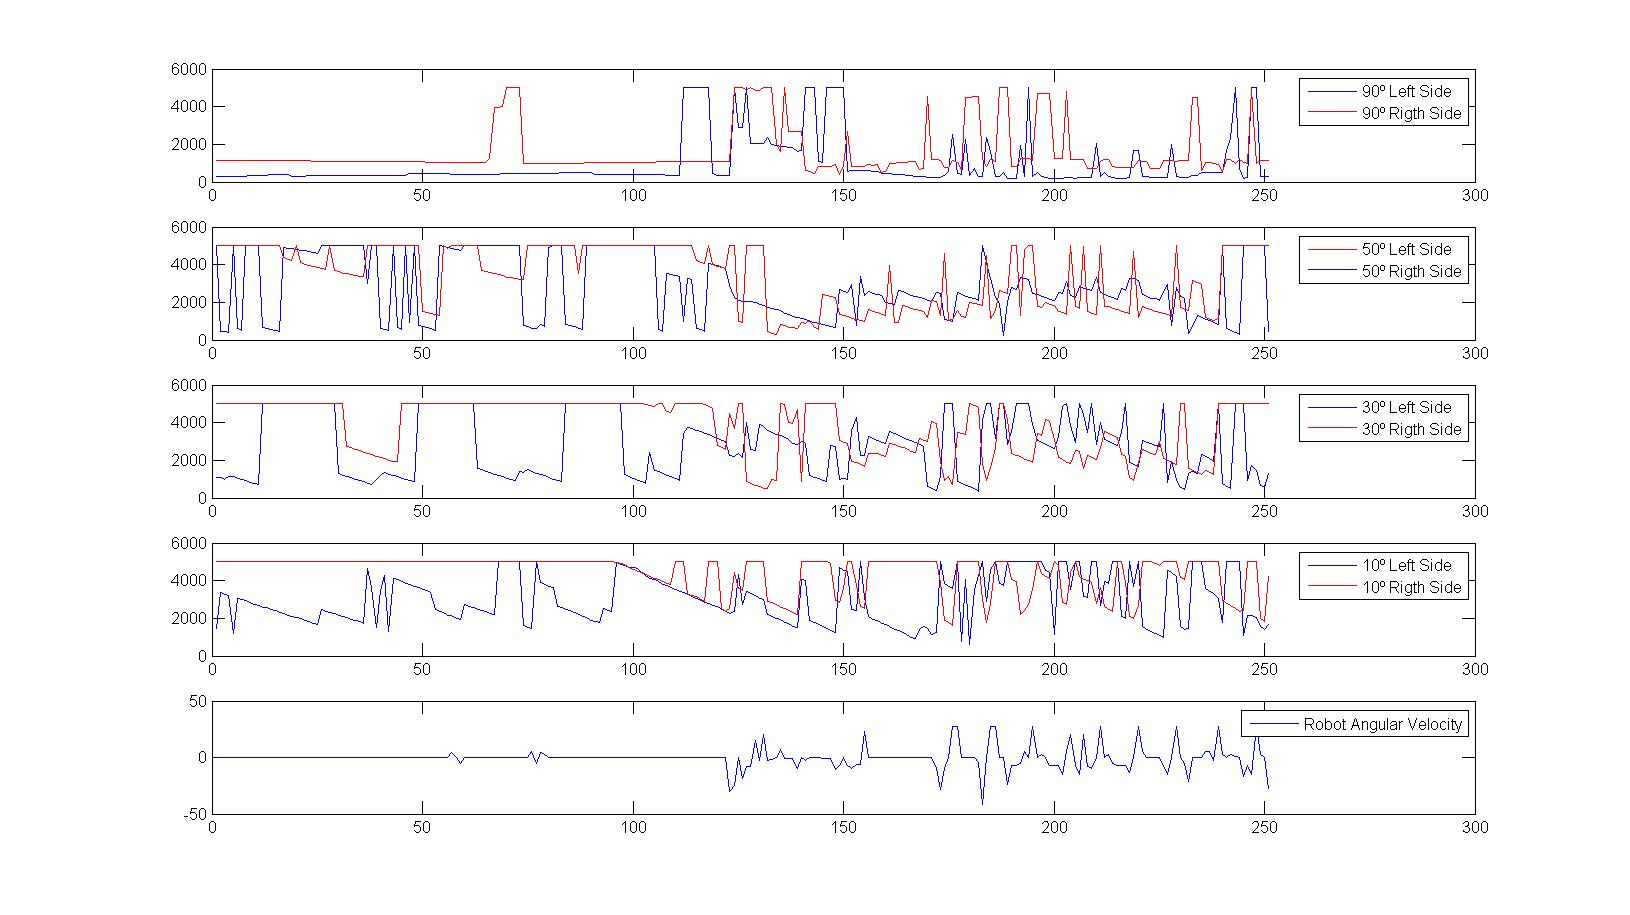
\includegraphics[width=0.7\linewidth]{sonar_map_section.jpg}
	\caption{Angular Velocity variation with the sonar signals.}
    \label{fig:sonar_map}
\end{figure}

These sonar readings were obtained in the section of the path shown in \ref{fig:sonar_map_section}. It's possible to see how, when the sonars from the left side (10\degree, 30\degree, 50\degree) go below 350 mm, the the angular velocity has a compensation to the right. The inverse happens when the equivalent sonars on the right side have readings below 350 mm.

In the case of the 90\degree sonars, besides turning away from the wall when they read a distance under 250 mm, if the distance read is under 450 mm and there isn't any warning from one of the other sonars the robot moves in a straight line with the same orientation as before. This was a defensive measure to prevent any trajectory corrections that would turn the robot towards the obstacle or a wall and lead to a collision.

\begin{figure}[H]
	\centering
	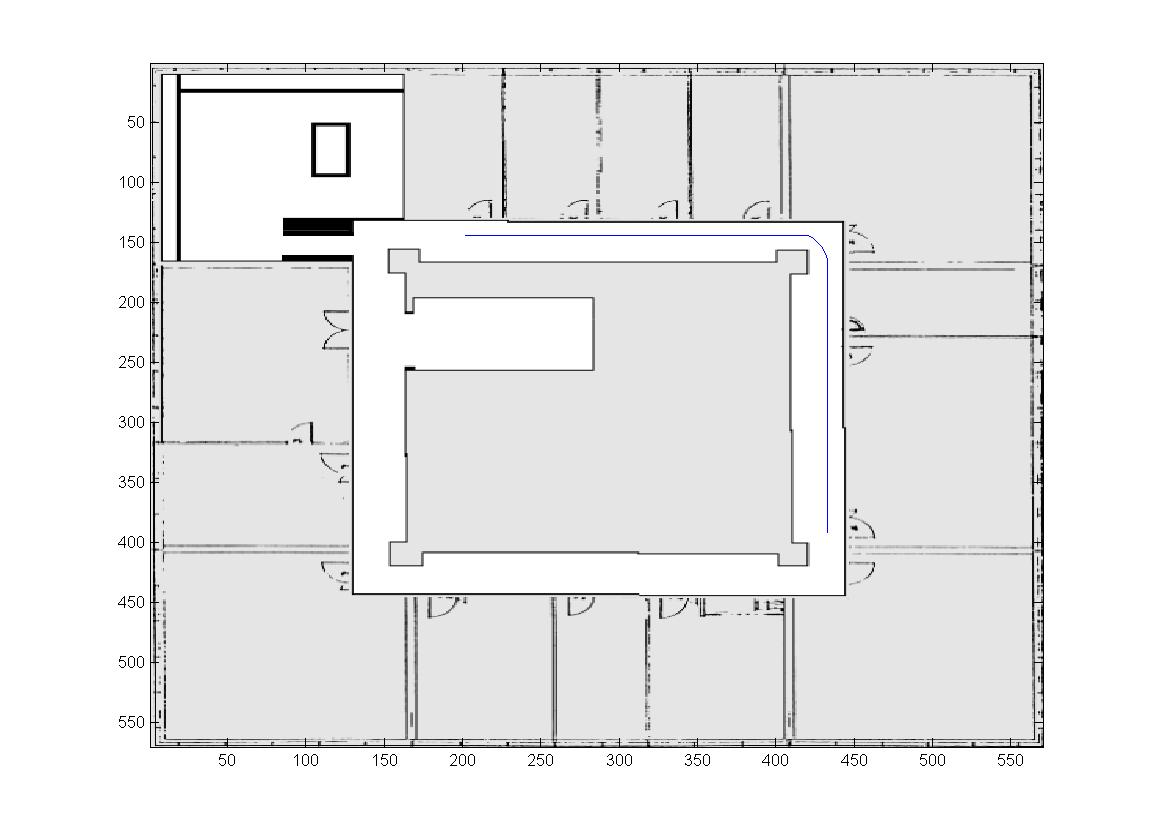
\includegraphics[width=0.7\linewidth]{sonar_map_used_section.jpg}
	\caption{Section of the path used to show how the sonar readings influence the angular velocity of the robot.}
    \label{fig:sonar_map_section}
\end{figure}

With these analysis we can conclude that even though the robot wasn't able to enter the laboratory and return to the starting position, the developed control program was capable of taking the robot out of the laboratory and driving it around the fifth floor without letting the robot hit any obstacle in the way (whether a static obstacle like a bench or a door, or a dynamic obstacle such as a person that would get in the way of the robot planned trajectory). With these results we consider that the program behaved positively and that if we had a little more time to correct some minor problems (namely that, during the trajectory, the robot would lose 2 m), the robot would be able to return to the laboratory and reach the starting position.

\section{Conclusion}
From what was shown in this report, we can conclude that although in simulation our control program works correctly and the robot shows a smooth movement and convergence to the reference trajectory, the results of the robot field tests weren't so positive, since the robot couldn't complete the lap around the fifth floor and return to its staring position in the laboratory.

One possible justification for this is that we didn't compensate correctly the odometry errors and, when they accumulated, the robot started to make the calculations with wrong trajectory points causing that it couldn't make the turn to enter the laboratory and finish the trajectory in the starting point.

Another possible justification is that when we prevented the errors to go higher than a certain value, we were in fact adding a little error to the robot calculations each time that occurred. The 2 m that it lost during the lap may be in fact a consequence of that error accumulation.

Future work to be done with this program would be to carefully check if those two possible reasons were in fact the motives for which the robot couldn't return to the laboratory and to its starting point or if there are other reasons that we haven't envisaged. One of the solutions that could be implemented to better our results is the usage of odometry filters that would correct the readings from the sensors, which we weren't capable of introduce due to lack of possibility to investigate the area.

Even though the robot with our control program couldn't return to the starting point, we consider that the results are positive, because, as we have shown, the robot can reach the laboratory entrance after performing a lap around the fifth floor and, in the simulation, the results show that the theoretical principles of our program are correct. Thus, we believe that the problem was related to the odometry readings and perhaps with a little more time we could have achieved total success.

\end{document}